다음 그림과 같이 $\overline{\mathrm{AB}} = \overline{\mathrm{AC}}$인 직각이등변삼각형 $\mathrm{ABC}$의 꼭짓점 $\mathrm{A}$를 지나는 직선 $l$이 있다. 두 꼭짓점 $\mathrm{B}$, $\mathrm{C}$에서 직선 $l$에 내린 수선의 발을 각각 $\mathrm{D}$, $\mathrm{E}$라 하자. $\overline{\mathrm{BD}} = 10\,\mathrm{cm}$, $\overline{\mathrm{CE}} = 8\,\mathrm{cm}$일 때, 삼각형 $\mathrm{ABC}$의 넓이는 몇 $\mathrm{cm}^2$인지 구하여라.

\begin{figure}[h]
\centering
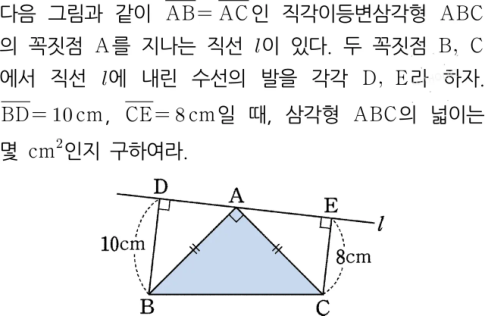
\includegraphics[width=0.4\textwidth]{plain0_problem_04_figure.png}
\end{figure}
